% Source : http://forum.mathematex.net/latex-f6/axe-et-inequation-t11753.html#p113736

\documentclass{article}
	\usepackage{tikz}
	\usetikzlibrary{shapes,patterns}


\begin{document}

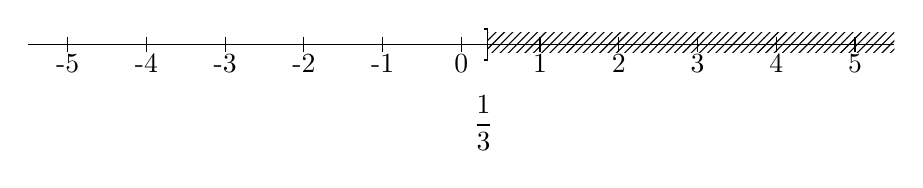
\begin{tikzpicture}[draw=black,xshift=5cm]
	\draw (-5.5cm,0cm)--(5.5cm,0cm);

	\foreach \i in {-5,...,5}{
		\draw[xshift=\i cm] (0cm,.1cm)--(0cm,-.1cm)
		node[yshift=-.15cm]{\i};
	}

	\path[pattern=north east lines]
		(0.333cm,-0.1cm)  rectangle (5.5cm,0.15cm);

	\draw[xshift=0.333cm,line width=0.7pt]
		(-0.05cm,0.2cm)--(0cm,0.2cm)--(0cm,-0.2cm)--(-0.05cm,-0.2cm)

	node[yshift=-0.8cm] {
		$\displaystyle\frac{1}{3}$
	};
\end{tikzpicture}

\end{document}
